\section{Geometric interpretation}
\begin{equation*}
\begin{split}
 \ket{\alpha} &\equiv \frac{1}{\sqrt{N-M}} \sum_{x}{}^{''} \ket{x} \\
 \ket{\beta} &\equiv \frac{1}{\sqrt{M}} \sum_{x}{}^{'} \ket{x}
\end{split}
\end{equation*}
\begin{equation*}
    \ket{\psi} = \sqrt{\frac{N-M}{N}} \ket{\alpha} + \sqrt{\frac{M}{N}} \ket{\beta}
\end{equation*}
\begin{equation*}
    \hat{G}\ket{\psi} = \cos\frac{3\theta}{2} \ket{\alpha} + \sin\frac{3\theta}{2} \ket{\beta}
\end{equation*}
\begin{equation*}
    \hat{G}^{k}\ket{\psi} = \cos\biggl(\frac{2k+1}{2}\theta\biggr) \ket{\alpha} + \sin\biggl(\frac{2k+1}{2}\theta\biggr) \ket{\beta}
\end{equation*}

\begin{figure}
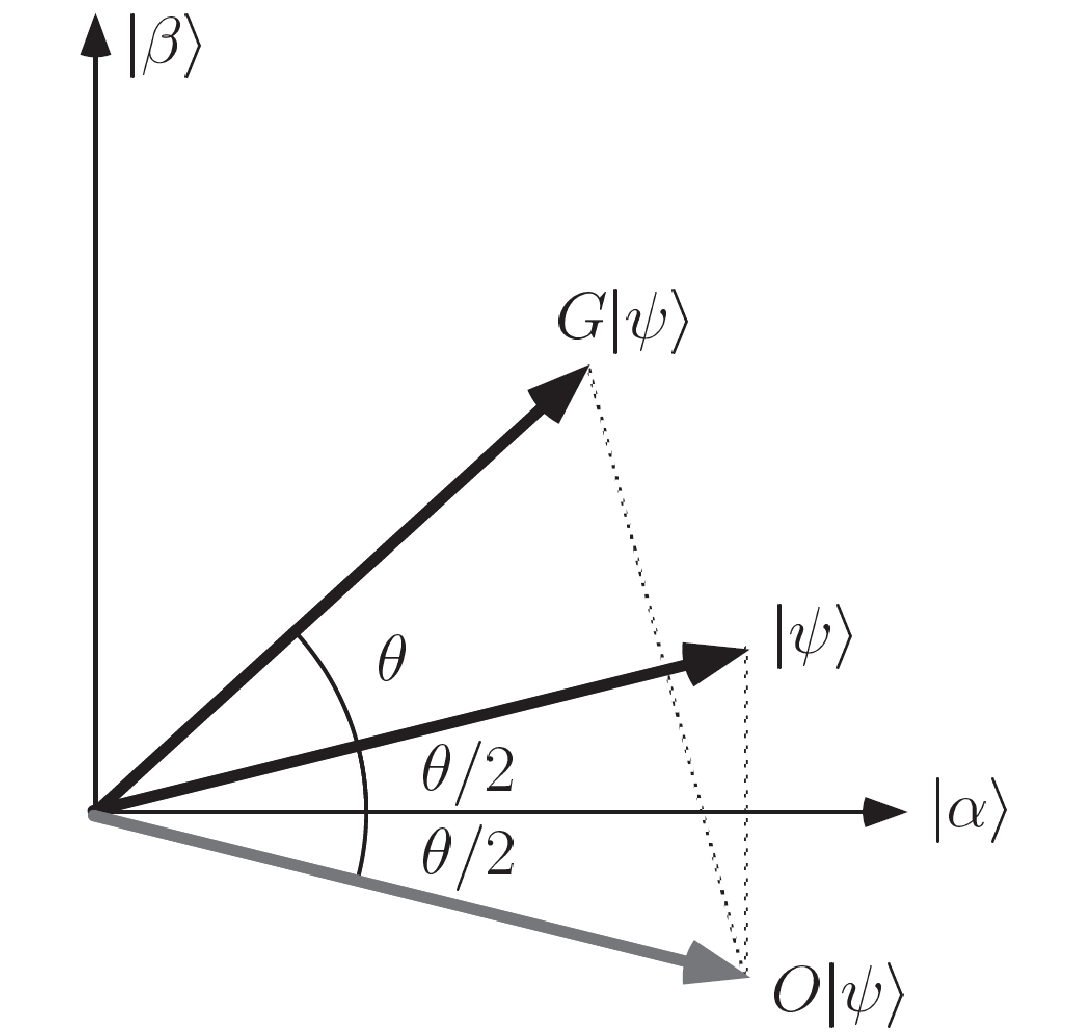
\includegraphics{geometric-interpretation.png}
\centering
\end{figure}

